%!TEX encoding = UTF-8 Unicode
%!TEX TS-program = pdflatex

%%% --- PREAMBLE --- %%%
\documentclass[a4paper,11pt]{article}

\usepackage[italian]{babel}
\usepackage[left=2cm,right=2cm,top=2cm,bottom=2cm,headheight=14pt]{geometry}
\usepackage[T1]{fontenc} % OT1: basic, T1: western, T3 and T5: exotic, T4: lots of characters but WORSE READABILITY
\usepackage[utf8x]{inputenc} % utf8x supports more characters than utf8
\usepackage{graphicx} % import PNG, JPG and PDF with \includegraphics
\usepackage[usenames,table]{xcolor} % \color
\usepackage{amssymb}
\usepackage{amsmath}
\usepackage{amsfonts}
\usepackage{float}
\usepackage{mathtools} % (!! PLACE BEFORE hyperref !!)
\usepackage{xfrac} % \sfrac
\usepackage{cancel} % \cancel \cancelto
\usepackage{hyperref} % interactive links in TOC, URLs and references
% unneded \usepackage{fixltx2e} % provides \textsubscript and makes some fixes
\usepackage[toc,page]{appendix}
\usepackage{siunitx} % \num \si \SI
\usepackage{alltt} % {alltt} (like verbatim but with commands)
\usepackage{moreverb} % {listing}
\usepackage{listings} % {lstlisting}
\usepackage[overload]{textcase} % fixes \MakeUppercase and \MakeLowercase
\usepackage[normalem]{ulem} % \uline \uwave \sout \xout
\usepackage{enumerate} % adds options for {enumerate}
\usepackage{paralist} % inline lists with {inparaenum}
\usepackage[official]{eurosym} % \euro
\usepackage{tabu} % {tabu} (like {tabular} with improvements)
\usepackage{layout} % layout description
\usepackage{multicol} % {multicols}
\usepackage{lipsum} % filling text generator with \lipsum
\usepackage[section]{placeins} % inhibits float figures from trepassing a section boundary
\usepackage{subfig} % \subfloat to be used inside {figure}
\usepackage{wrapfig} % {wrapfigure} (like {figure} but allows text to flow on its sides)
\usepackage{ifthen} % \ifthenelse
\usepackage{calc}
\usepackage{array}
\usepackage{multirow}
\usepackage{booktabs} % \toprule, \midrule, \bottomrule
\usepackage{fancyhdr}
\usepackage{wasysym}
\graphicspath{ {../Figs-Tabs/} } % graphics search directories
\setcounter{tocdepth}{1} % -1: part, 0: chapter, 1: section, 2: subsection, 3: subsubsection

\lstset{ %
	language=C,
	deletekeywords={},
	morekeywords={},
	backgroundcolor=\color{white},
	basicstyle=\ttfamily\small,
	commentstyle=\color{teal},
	keywordstyle=\color{magenta},
	stringstyle=\color{purple},
	identifierstyle=\color{violet!80!black},
	numbers=left,
	numbersep=7pt,
	numberstyle=\scriptsize\sffamily\color{gray},
	stepnumber=1,
	breakatwhitespace=false,
	breaklines=true,
	keepspaces=true,
	showspaces=false,
	showstringspaces=false,
	showtabs=false,
	tabsize=2,
	captionpos=none,
}

\newcommand{\ndr}[1]{\footnote{#1 (n.d.r.)}}

\newcommand{\fig}[1]{\figurename{ \ref{fig:#1}}} %inserting reference to figures
\newcommand{\tab}[1]{\tablename{ \ref{tab:#1}}} % inserting reference to tables
\newcommand{\eqn}[1]{equazione \eqref{eq:#1}} % inserting reference to equation

\newcommand{\dof}{\text{ dof}} % degrees of freedom
\newcommand{\paral}{\mathbin{\|}} % impedance parallel
\DeclareSIUnit\deca{decade} % decade unit definition for use in siunitx
\DeclareSIUnit\gauss{Gs} % Gauss unit definition for use in siunitx

\newcommand{\insertpart}[2]{\input{#1}}
\newcommand{\e}{\textbf{$e^{-}$}}

\sisetup{%
	separate-uncertainty = true,
	per-mode = symbol,
	bracket-numbers = false,
	multi-part-units = single,
	table-number-alignment = center,
	range-phrase = \text{--},
	range-units = single,
	output-complex-root =  \text{\ensuremath{j}},
	table-figures-decimal = 3,
	table-figures-exponent = 0,
	table-figures-integer = 2,
	table-figures-uncertainty = 2,
}

%%% --- DOCUMENT --- %%%


%%%%% SIunits example use:
% \si{\kilo\volt\per\meter\squared} -> kV/m^2
% \SI{1.222 (34)}{\joule\second}    -> 1.222 +- 0.034 Js
% \SI{1.222 \pm 0.034}{\nF}         -> 1.222 +- 0.034 nF
% use it plz

\pagestyle{fancy}
\author{Gruppo BF \\ Thomas Giannoni, Valerio Lomanto, Roberto Ribatti}
\title{Esercitazione N. 12: Flip-Flop e contatori}
\date{4 aprile 2017}

\author{Gruppo BF \\ Thomas Giannoni, Valerio Lomanto, Roberto Ribatti}
\title{Esercitazione N. 13: Macchine a stati finiti: semaforo }
\date{2 maggio 2017}

\begin{document}
\maketitle
\begin{abstract}
In quest'esperienza sono state realizzate  alcune macchine a stati finiti (FSM) che 
gestiscono un semaforo.
Le prime due macchine finite ivi riportate sono state realizzate con circuiti integrati; 
basandole su Flip-Flop D-Latch. La prima di esse implementa un semaforo costantemente abilitato, 
che alterni gli stati : 

Verde acceso $\longrightarrow$ Verde e 
giallo acceso $\longrightarrow$ rosso acceso $\longrightarrow$ 
verde acceso  ciclicamente.

La seconda FSM realizzata con 
circuiti integrati riprende la precedente introducendo un segnale di abilitazione; 
con il semaforo disabilitato sono stati imposti gli stati:

 Led giallo acceso $\leftrightarrow$ Led giallo spento.

Nella seconda fase dell'esperienza è stato realizzato un programma che attraverso ARDUINO
 implementi il semaforo abilitabile.
\end{abstract}

\section{Strumentazione}
	In questa esperienza sono state impiegati:
	\begin{itemize}
		\item alcuni circuiti integrati:
		\begin{enumerate}
			\item 1 IC SN74LS00 (Quad NAND Gate);
			\item 2 IC SN74LS74 (Dual D-Latch);
			\item 1 IC SN74LS08 (Quad AND Gate);
			\item 1 IC SN74LS2 (Quad OR Gate);
		\end{enumerate}
		\item 1 Switch a 4 bit;
		\item 3 diodi LED; rispettivamente verde giallo e rosso
		\item il generatore di onde quadre basato su Arduino realizzato precedentemente.
	\end{itemize}
\section{Semafori con circuiti integrati }
Il semaforo può presentare la modalità ABILITATO e DISABILITATO. Qualora sia abilitato si deve 
ottenere Verde acceso $\longrightarrow$ Verde e 
giallo acceso $\longrightarrow$ rosso acceso $\longrightarrow$ 
verde acceso  ciclicamente. Mentre qualora il semaforo sia disabilitato si deve ottenere
Led giallo acceso $\leftrightarrow$ Led giallo spento.
Per descriminare tra i due modalità di funzionamento può essere impiegato un segnale di abilitazione 
ENABLE (E).
Per la realizzazione del semaforo è stato realizzato d'apprima un semaforo privo di enable , per cui il sistema risulti costantemente abilitato;
dopodiché riprendendone lo schema circuitale si è introdotto il segnale di ENABLE.
\paragraph{Semaforo privo di enable}
Per la realizzazione una FSM che alterni gli stati come in \figurename{\ref{fig:stati}}
Avendo tre stati diversi è stato necessario impiegare una codifica a 2 bit.
Essendo la codifica arbitraria si riporta la codifica impiegata in 
\tablename{\ref{tab:cod}}.
Essendo possibile con due bit ottenere anche lo stato 11,  non corrispondente a nessuno degli stati codificati,
è stato imposto che dallo stato ROSSO sul successivo fronte di salita di clock il segnale costituisca
un reset forzando pertanto la transizione \\ROSSO $(1;0)$  $\longrightarrow$ VERDE $(0;0)$.
Rendando pertanto il lo stato 1;1 quale inaccessibile.
Si riporta la \tablename{ \ref{tab:tran}} delle transizioni tra i vari stati della FSM.

Dalla \tablename{ \ref{tab:tran}} si ottiene  $b_{1}^{n+1} = \overline{b_{1}^{n}} \cdot b_{0}^{n}$ e $b_{0}^{n+1} = \overline{b_{1}^{n}} \cdot \overline{b_{0}^{n}}$
\\
\\
SCRIVERE CHE TIPO DI MACCHINA é
\\
\\
Per realizzare la FSM basata sugli integrati a disposizione, e che realizzi quanto appena descritto,
 è stato realizzato il circuito in \figurename{ \ref{fig:sem1}} alimentando la componentistica con una tensione 
 $V_{cc}=$\SI{0.1 \pm 456456215}{\volt}.Si segnala inoltre che in serie con i led sono state montate delle resistenze $R\sim 330$\si{\ohm} per limitare la richiesta di corrente.
\begin{figure}[h!]
	\begin{minipage}{0.5\textwidth}
		\centering
		\includegraphics[scale=0.20]{immagineM.png}
		\caption{Stati della FSM semaforo senza En.}
		\label{fig:stati}
	\end{minipage}
\begin{minipage}{0.5\textwidth}
	\centering
	\begin{tabular}{ssc}
	\toprule
	b_{1} & b_{0} & stato corrispondente\\
	\midrule
	0 & 0 & VERDE\\
	0 & 1 & GIALLO \& VERDE\\
	1 & 0 & ROSSO\\
	1 & 1 &  X (NON VOLUTO)\\
	\bottomrule
	\end{tabular}
	\caption{Codifica degli stati impiegati}
	\label{tab:cod}
\end{minipage}
\end{figure}


\begin{table}[h]
\centering
\begin{tabular}{ss|ss|sss}
	\toprule
	b_{1}^{n} & b_{0}^{n}  & b_{1}^{n+1} & b_{0}^{n+1} & \text{LED VERDE} & \text{LED GIALLO} & \text{LED ROSSO} \\
	\midrule
	 1 & 1 & 0 & 0 & x & x& x\\
	 0 & 1 & 1 & 0 & 1 & 1& 0\\
	 1 & 0 & 0 & 0 & 0 & 0& 1\\
	 0 & 0 & 0 & 1 & 1 & 0& 0\\
	\bottomrule
\end{tabular}
\caption{Tabella delle transizioni della FSM semaforo sempre abilitato.
Il segnale $1$ corrisponde al LED acceso, $0$ LED spento.
Lo stato $b_{1}=1$ $b_{0}=1$ deve risultare inaccessibile. }
\label{tab:tran}
\end{table}

\begin{figure}[h!]
		\centering
		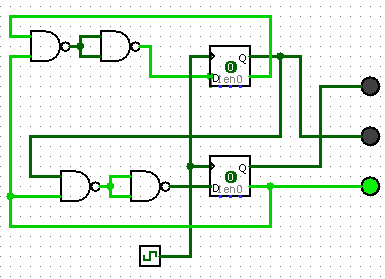
\includegraphics[scale=1.0]{circ1.png}
		\caption{Circuito che realizzi il semaforo senza En.}
		\label{fig:sem1}
	\end{figure}

Per la verifica del funzionamento circuitale è stato 
 inviato un segnale di clock di frequenza bassa, $f\sim $\si{\hertz} e effettuando un primo controllo attraverso l'accensione dei LED. Si è successivamente aumentata la frequenza di clock $f= $\SI{.0000001\pm 45}{\hertz}
 ed acquisito i valori di tensione corrispondente alle uscite dei vari LED, riportate in 
 \figurename{ \ref{fig:acq}}. Dall'osservazione di
  tali acquisizioni si verifica l'accordo con le specifiche attese. 
 
\begin{figure}[h]
	\centering
	\subfloat[clock ch.  LED VERDE ch]{
		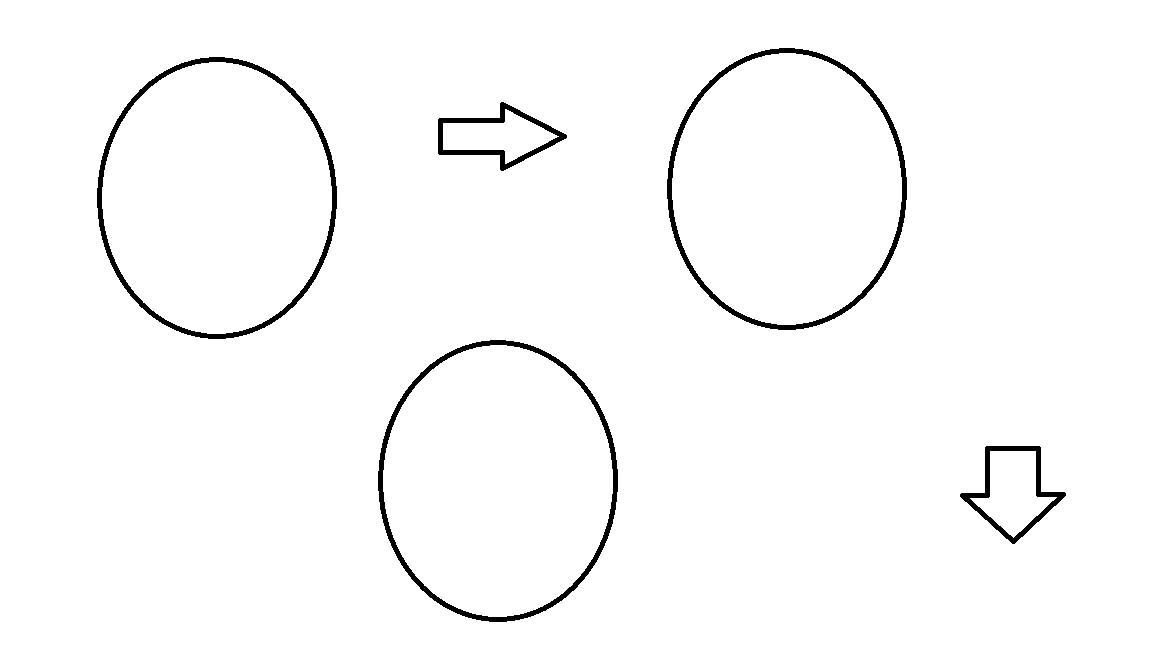
\includegraphics[scale=0.3]{Immagine.png}
	}
	\subfloat[clock ch. LED GIALLO ch]{
		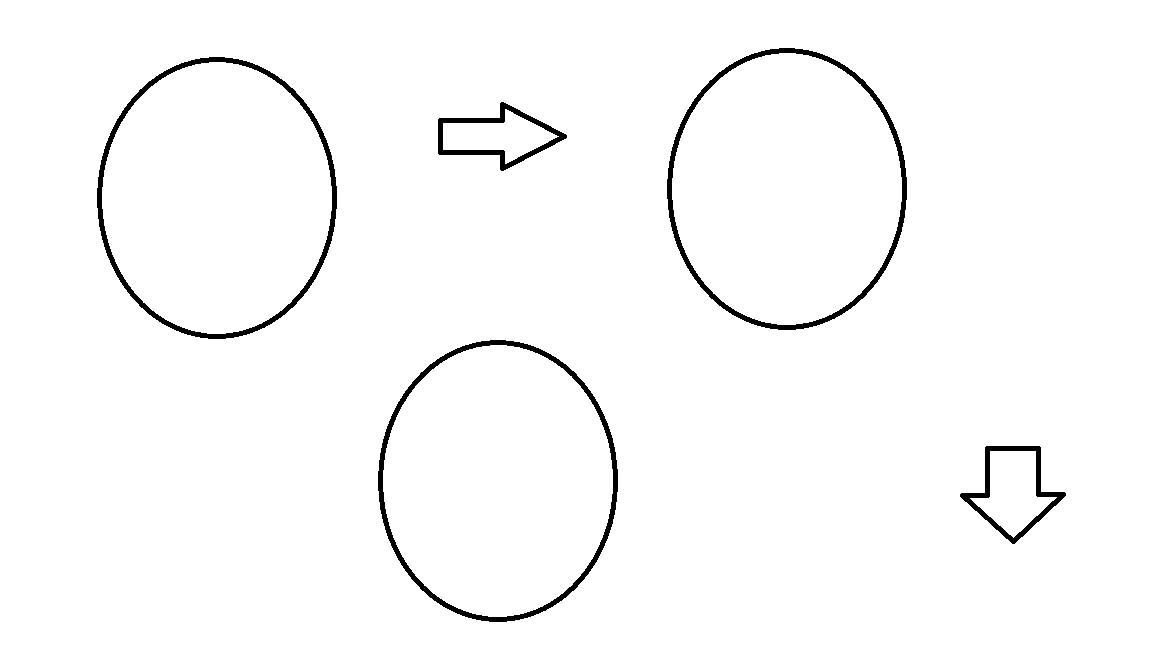
\includegraphics[scale=0.3]{Immagine.png}
		}\\
	\subfloat[clock ch.  LED ROSSO ch]{
		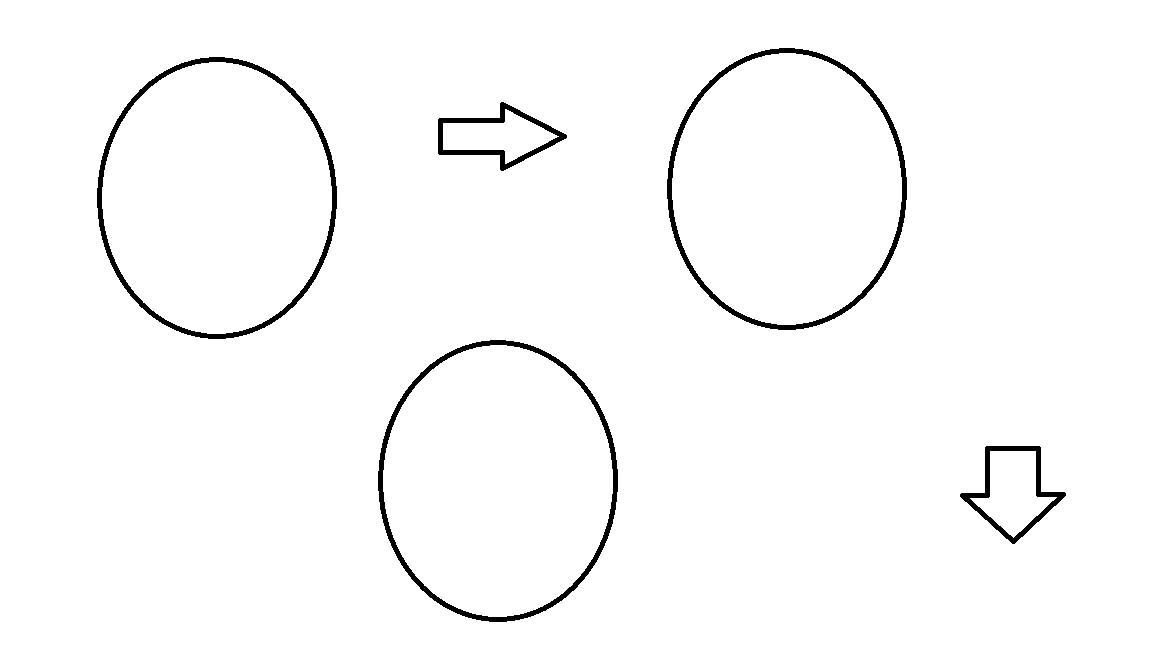
\includegraphics[scale=0.3]{Immagine.png}
		}
	\subfloat[clock ch.  $b_{0}$ ch]{
		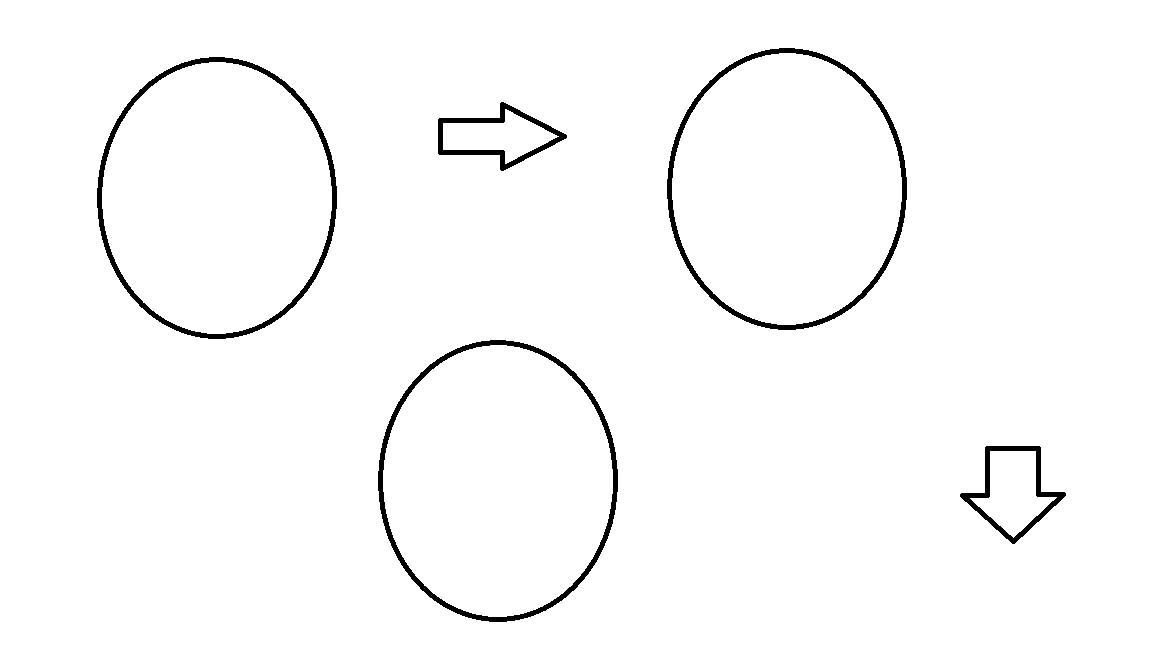
\includegraphics[scale=0.3]{Immagine.png}
		}\\
	\subfloat[clock ch. $b_{1}$  ch]{
		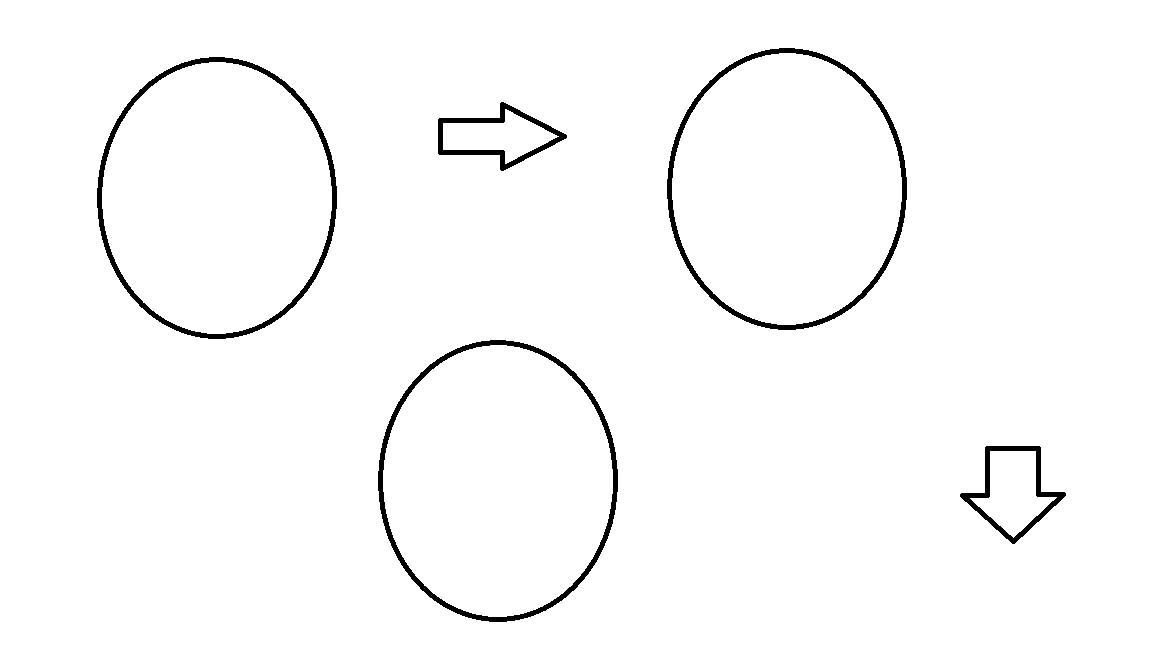
\includegraphics[scale=0.3]{Immagine.png}
	}
\caption{Acquisizione telle tensioni osservate nel semaforo privo di ENABLE}
\label{fig:acq}
\end{figure}
\paragraph{Semaforo completo}
	\end{document}
